% THIS IS SIGPROC-SP.TEX - VERSION 3.1
% WORKS WITH V3.2SP OF ACM_PROC_ARTICLE-SP.CLS
% APRIL 2009
%
% It is an example file showing how to use the 'acm_proc_article-sp.cls' V3.2SP
% LaTeX2e document class file for Conference Proceedings submissions.
% ----------------------------------------------------------------------------------------------------------------
% This .tex file (and associated .cls V3.2SP) *DOES NOT* produce:
%       1) The Permission Statement
%       2) The Conference (location) Info information
%       3) The Copyright Line with ACM data
%       4) Page numbering
% ---------------------------------------------------------------------------------------------------------------
% It is an example which *does* use the .bib file (from which the .bbl file
% is produced).
% REMEMBER HOWEVER: After having produced the .bbl file,
% and prior to final submission,
% you need to 'insert'  your .bbl file into your source .tex file so as to provide
% ONE 'self-contained' source file.
%
% Questions regarding SIGS should be sent to
% Adrienne Griscti ---> griscti@acm.org
%
% Questions/suggestions regarding the guidelines, .tex and .cls files, etc. to
% Gerald Murray ---> murray@hq.acm.org
%
% For tracking purposes - this is V3.1SP - APRIL 2009

\documentclass{acm_proc_article-sp}

\usepackage{url} % for url citation
\usepackage{epstopdf}

\begin{document}

\title{Towards Non-Consumptive Cloud Computing for Digital Humanities}

\author{}

\maketitle
\begin{abstract}
As the amount of digitized archives grows, compute technology plays an increasing important role in digital humanities research. The advent of cloud computing offers researcher computation capabilities to process tens of thousands of archives which goes beyond their desktop machines can process. However, for copyrighted archives, it poses security challenges to the compute platform. In this paper, we investigate non-consumptive research, a research that allows user access copyrighted archives while prevents archives reconstruction during user access, in cloud computing. We build an infrastructure as a service (IaaS) cloud framework that makes use of data capsule to enforce non-consumptive research policy in virtual machine. This paper presents our architecture design and implementation details, and outlines next steps for future development.
\end{abstract}

% A category with the (minimum) three required fields
\category{H.3.4}{Systems and Software}{Distributed systems}[cloud computing, data capsule]
%A category including the fourth, optional field follows...
\category{K.6.m}{Miscellaneous}{Security}[non-consumptive research]

\terms{Architecture, Design, Implementation}

\keywords{Cloud computing, Non-consumptive research, data capsule} % NOT required for Proceedings

\section{Introduction}
As the amount of digitized archives keeps growing, researchers of digital humanities are facing with materials that they could ever hope to read in life time. For example, some researchers checked some of Ian Watt's claims against 3,600 novels between 18th and 19th century \cite{Example}. It is tedious, if possible, for human being to do this task by hitting the library stacks, checking out books and examining book contents. Therefore, digitized archives with computer access significantly changes the way digital humanities researchers perform research. Computer technology has been applied to facilitate digital humanities research on massive digitized materials. For instance, researchers run topic modeling algorithm on a set of digitized books to identify common topics among books \cite{LDA}, which cannot be discovered easily by just reading the books.

However, the massive amount of digitized texts also poses challenges on data analysis. First, compute capabilities required vary and depend on the analysis tasks as well as amount of texts. For example, running topic modeling algorithm generally requires more CPU cycles and memory than generating a word cloud based on word frequency. Fixed hardware setting of user desktop is not suitable to deal with such dynamic workloads. Second, high performance computing(HPC) provides a way for user to allocate resource dynamically based on her workload. However, HPC is batch oriented and digital humanities researchers usually need an interactive way to access the compute resources. Thus cloud computing is preferred in such case. Third, some of the digitized contents are copyrighted. Allowing user algorithms run directly on copyrighted texts opens a vulnerable channel that non-consumptive constraint may be violated. According to \cite{BookSettlement}, non-consumptive research is a research that no action or set of actions on the part of users, either acting alone or in cooperation with other users over the duration of one or multiple sessions can result in sufficient information gathered from a collection of copyrighted works to reassemble pages from the collection. In other words, a user may steal copyrighted content while she runs her algorithm. We extend the definition above to include the situation that a user computer is compromised by malicious programs which acts on user\rq s behave to steal copyrighted content.

We propose a non-consumptive cloud framework to address challenges mentioned above. On one hand, cloud computing, which has elastic computing feature, is a natural fit for various analysis tasks. Researcher can create virtual machines shipped with different compute capabilities based on the need. Once the analysis is done, virtual machine is wiped out and resources are released for other users to share. On the other hand, the virtual machine of our framework is equipped with data capsule \cite{Borders:2009:PCD:1855768.1855791} to provide non-consumptive policy to prevent copyrighted leakage under the assumption that virtual machine is compromised. In data capsule, one virtual machine has two modes, i.e. maintenance mode and secure mode. In maintenance mode, user can access network and install software freely, but cannot access copyrighted texts. In secure mode, copyrighted texts become accessible to user while network access and file system access are highly constrained. Users are only allowed to access a predefined set of network addresses and write to a specific volume which is only visible in secure mode. Every other changes user made to the system in secure mode, except for the ones made to special volume, is lost when mode is switched from secure to maintenance. This is guard against the situation that copyrighted texts is saved in VM in secure mode and copied out through network in maintenance.

Our framework is implemented as a sub system within HathiTrust Research Center (HTRC) \cite{HTRC}. HTRC aims at enabling computational access for nonprofit and educational users to perform research on digitized texts. Through various services and tools provided from HTRC, user can access digitized texts, and run text mining algorithms on HTRC compute resources.

This paper is organized as follows. Section \ref{title:related} summaries related work. Section \ref{title:overview} presents an overview of HTRC and data capsule, and identifies the design requirements for our system. Section \ref{title:design} describes details of our system design and implementation. Section \ref{title:future} outlines future work and section \ref{title:conclusion} concludes.


\section{Related Work} \label{title:related}

Researchers have already leveraged the power of cloud computing in digital archives. Teregowda et al. employed cloud computing as underlying infrastructure for CiteSeerX, which is a public search engine and digital library for scientific and academic papers \cite{Teregowda:cloud}. Rosenthal et al. investigated the usage of cloud in their digital preservation system -- LOCKSS for libraries \cite{Rosenthal:preservation}. Our system differs from those systems in the sense that we investigate and promote non-consumptive research in the cloud platform.

Generally speaking, cloud computing can be categories as SaaS (software as a service), PaaS (platform as a service), and IaaS (infrastructure as a service) \cite{Armbrust:EECS-2009-28}. Our cloud framework intends to provide a weaker form of IaaS (infrastructure as a service). That is user can configure some of the VM specs, e.g., operation system, number of CPU, memory, and disk, but not the network, nor the volume. There are numbers of existing cloud platforms support IaaS, either in a commercial way or in an open source way. Amazon EC2 \cite{EC2} is probably the most well-known IaaS platform.  On regard to open source cloud platform, Eucalyptus \cite{Nurmi:2009:EOC:1577849.1577895} is an open source IaaS platform that provides Amazon compatible cloud environment. OpenStack \cite{OpenStack} is another open source IaaS platform that gains increasing popularity. Researchers investigated different cloud platforms \cite{Sempolinski:cloud,vonLaszewski:2012:CMC:2353730.2353779}. The reasons we do not build our system on existing open source platforms are two folds. First, existing cloud platforms introduce numerous complexities for the data capsule which enforces non-consumptive research policy in VM. Those complexities are from unnecessary features for digital humanities researchers. For example, researcher does not need to configure a software defined network to run her text mining algorithms. Second, existing cloud platforms are designed for general purpose and expose many vulnerable channels. For example, allowing user to configure network would pose significant threats to our systems. Therefore, instead of using existing cloud platform, we build a cloud framework around data capsule, which satisfies digital humanities researchers\rq need and non-consumptive research requirement. Our research also illuminates the path that data capsule could potentially be applied to more general cloud platforms.

Related work of Data Capsule.



\section{Overview} \label{title:overview}
This section presents background of HathiTrust Research Center (HTRC), data capsule and identifies threat model as well as design requirements for our system.

\subsection{HathiTrust Research Center Background} \label{subtitle:background}
HTRC consists of number of services that facilitate nonprofit and educational users to access and research on texts from HathiTrust Digital Library. Figure \ref{fig:htrc} below shows an overview of HTRC from an interaction point of view. HTRC provides users with a complexity hiding interface, left bar on Figure \ref{fig:htrc}, which shadows HTRC service complexity. The central cloud shape represents the entire HTRC system which can be divided into 4 categories: 1) metadata and data subsystem which provide metadata, raw text, and statistical information access; 2) data mining subsystem that embraces several tools for users to mine corpus; 3) job execution subsystem that runs various text mining algorithms on HPC environment; 4) auxiliary services subsystem that supports other services, e.g., user authentication service.

\begin{figure}[h]
  \centering
  \includegraphics[scale=0.3]{figures/htrc}
  \caption{HathiTrust Research Center Infrastructure.}
  \label{fig:htrc}
\end{figure}

\subsection{Threat Model}

The system is designed to allow user to access copyrighted data in a compromised operating system which runs in a virtual machine (VM). Neither the operating system, the driver, nor the applications (except for user�s application running against HTRC Data service) are trusted. Although our system allows arbitrary behaviors in VM, it does require some trusted components. The virtual machine monitor (VMM) that runs virtual machines is part of the trusted computing base (TCB). The hosts where VMM locates are also part of the TCB. The internal network among VMs is part of the TCB, i.e., firewall policy is sufficient to prevent attack from one VM to another one. User�s application that runs against HTRC Data service is considered trustworthy, although it could potentially encode the copyrighted data and deliver it as final result. We require user to sign a legal agreement before she uses our system. We intend to add some result analysis to automatically detect data leakage and leave this as future work.

\subsection{Data Capsule}

The data capsule was developed by Borders et al. \cite{Borders:2009:PCD:1855768.1855791}. It enforces two modes on a single virtual machine, i.e., maintenance mode and secure mode, to provide secure access to sensitive data. In maintenance mode, user is free to access internet and install software in VM. While in secure mode, sensitive data stored in a secure volume will be attached to the VM and become visible to user. The network access is blocked in secure mode to prevent data leakage by network. When user switches from secure mode to maintenance mode, changes made to places other than volume are wiped out so that sensitive data cannot leak through copying to local disk neither. Only changes made to volume is persistent. Therefore, in data capsule, user can access sensitive data and leakage cannot take place neither through network channel nor through disk.

Data capsule was mainly developed for general usage in single machine. We adapt and extend data capsule based on the context of HTRC. Sensitive data in HTRC is copyrighted text which is exposed through a API in Restful web service instead of staying in volume. Data capsule needs to enable the network channel between web service serving data and virtual machine. On regard to future HTRC services, data capsule should have a flexible network control mechanism. Besides, to carry out analysis tasks, researchers need persistent storage to store temporal results for iterative analysis purpose. Thus, the role of secure volume in data capsule is changed from mainly serving read to mainly serving write. In addition, data capsule is designed to work in single machine. To provide a cloud environment across multiple machines to multiple researcher, we need another layer on top of data capsule to coordinate different machines. We propose a web service layer, which is responsible for management effects e.g., resource allocation, request scheduling, status maintenance, and etc, on top of the data capsule to implement the cloud environment. Section \ref{title:design} gives details of design and implementation of data capsule in HTRC context.

\subsection{Design Requirements} \label{subtitle:requirement}
Our non-consumptive cloud framework falls into the second category mentioned in section \ref{subtitle:background} through provisioning a secure environment for user to conduct research against our data, probably copyrighted. We target digital humanities researchers and aim at providing a user friendly environment for user to access copyrighted text while preventing copyrighted text leakage. We identify following design requirements.
\begin{enumerate}
  \item It provides a cloud environment that makes better use of our backend resources;
  \item It prevents texts copied out from our system through network, and interference among users;
  \item It audits users activities;
  \item It is easy for researchers to use. Researchers have the privilege to configure the software and hardware environment to meet their needs;
  \item It can support large scale data process paradigm, e.g., MapReduce.
\end{enumerate}

\section{Design and Implementation} \label{title:design}
This section presents the details of the architecture and implementation of our system.

\subsection{Architecture}

Figure \ref{fig:architecture} delineates our architecture design. It consists of three layers, physical layer, web service layer and web front end layer from bottom to top. The physical layer includes physical machines and hypervisor software that run virtual machines. It also includes the data capsule implementation which is scripts that wrap hypervisor commands to perform multiple tasks. Database, image store and volume store also sit in this layer. Database is used by the web service to maintain persistent states for virtual machines and different operations. Virtual machine images as well as secure volumes locate in NFS, a share file system. The web service layer is the central controller of the system. It is responsible for resource allocation, request scheduling, state maintenance, and failover on physical layer. It also has an audit component to log user activities. Finally we expose the system through the web font end layer. It consists of a web UI where user interacts with our system and a user authentication server which validates user identification. To validate user identity, we use OAuth 2.0 \cite{OAuth2} for user authentication.

\begin{figure}[h]
  \centering
  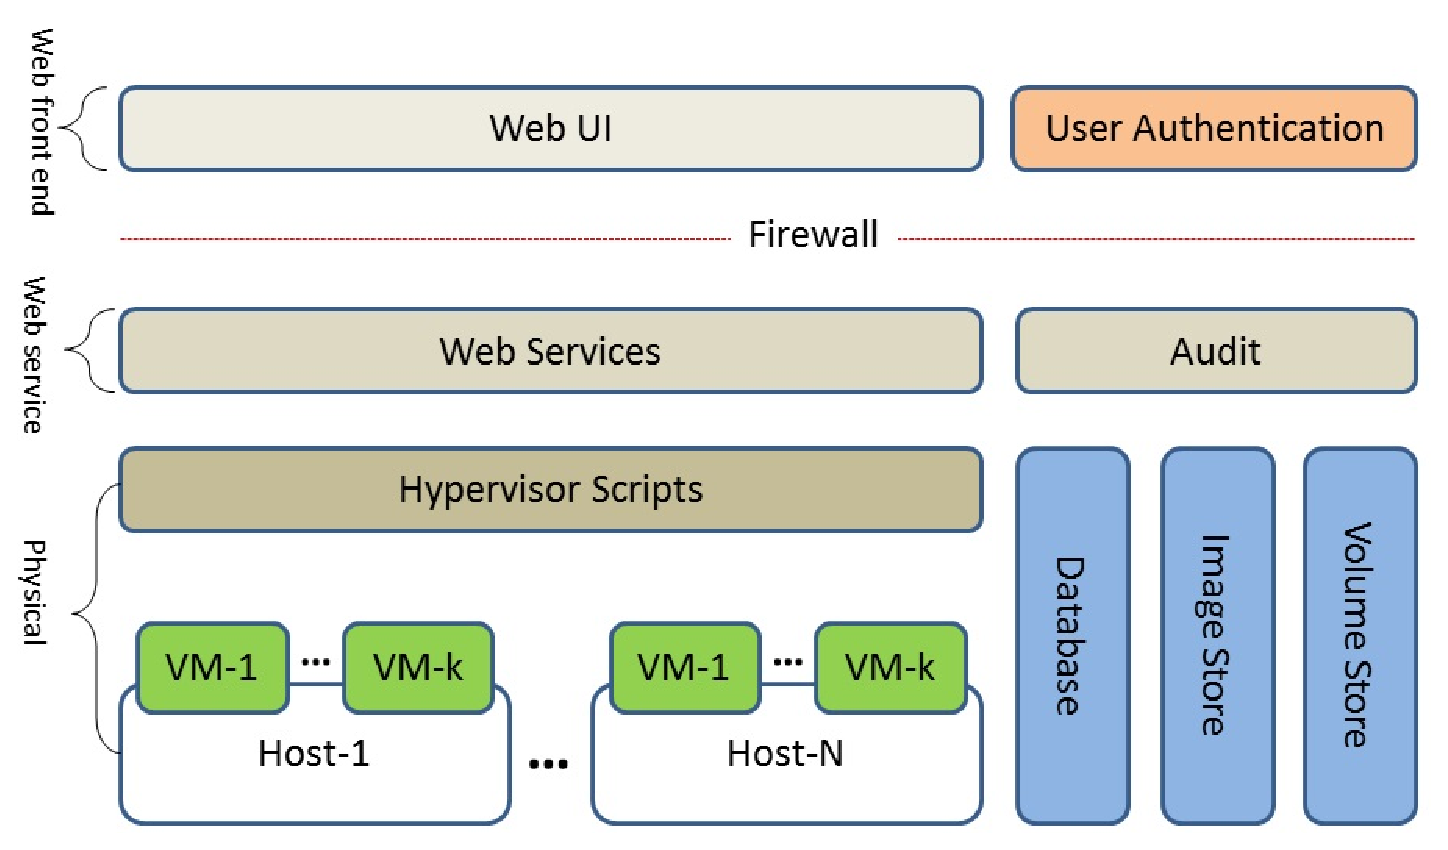
\includegraphics[scale=0.33]{figures/layers}
  \caption{Overall architecture design.}
  \label{fig:architecture}
\end{figure}


\subsection{Workflows}
This section presents control flows within our system components.

\subsubsection{Virtual machine operations} \label{subsubtitle:control}
Figure \ref{fig:control} describes the control flow in our system. First user logs into web UI, which delegates the authentication to OAuth 2 server which validates user login credentials. Details of user authentication is presented in section \ref{subsubtitle:auth}. Upon validation success, user can manipulate the VM through the web UI. We use VM creation request as an example here. The UI forwards the request along with an authentication token to web service. When web service receives the request, it validates the token against OAuth 2 server again. The reason for double validation is web UI might be compromised and web service needs to validate requests coming from web UI. If validation successes, web service will prepare to invoke corresponding hypervisor script. It makes scheduling decision on which host to launch VM, allocates ports for VM, retrieves image information from database, and etc. Once the preparation is done, it will call hypervisor script remotely to launch a VM on a particular host, monitor the response and update VM state in database. Meanwhile web service will return user the information required to log into VM, e.g., VNC port. Other VM operations (shutdown, delete, launch, switch mode from one another) follow the same path described above.

\begin{figure}[h]
  \centering
  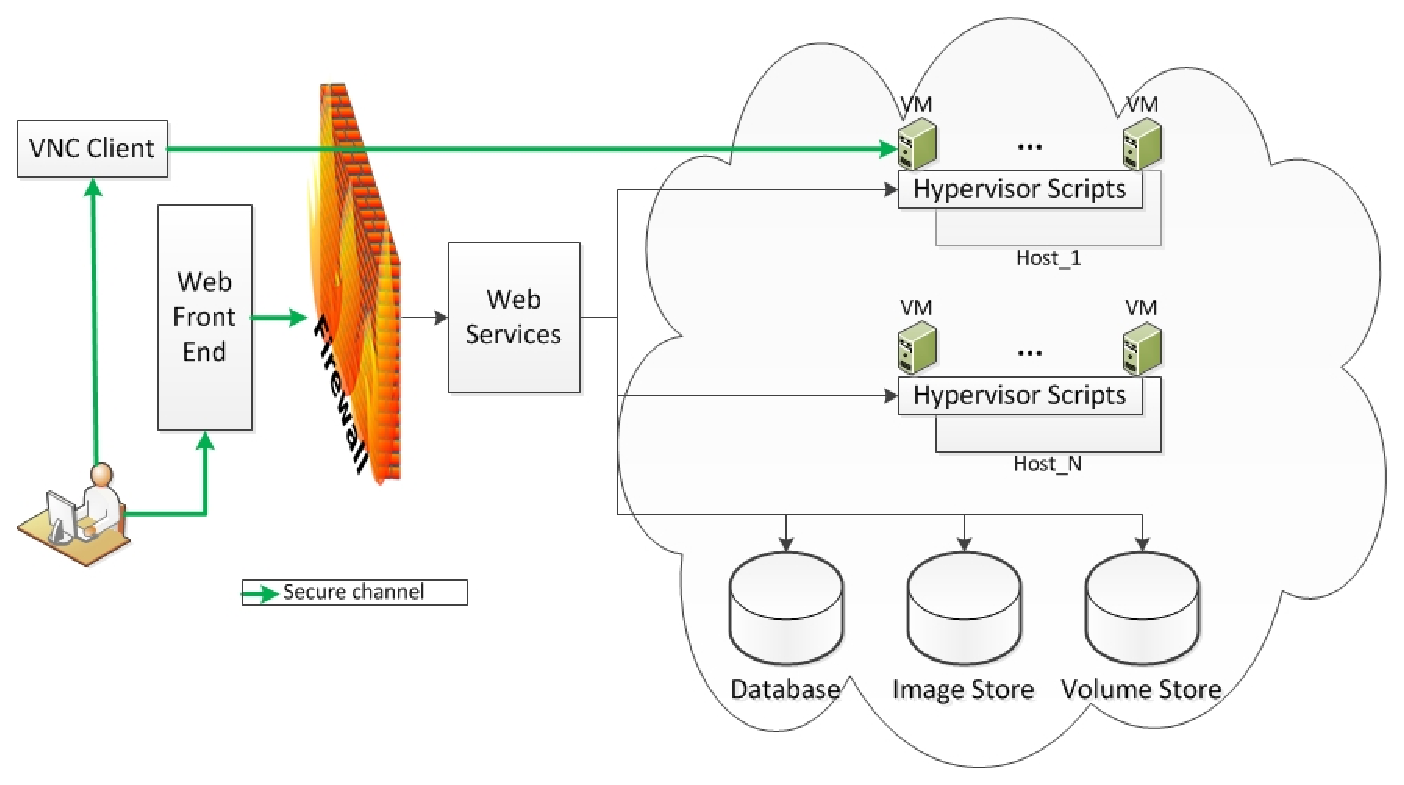
\includegraphics[scale=0.35]{figures/workflow-control}
  \caption{System control flow.}
  \label{fig:control}
\end{figure}

\subsubsection{Authentication} \label{subsubtitle:auth}
We use OAuth 2.0 as our authentication protocol \cite{OAuth2}. A dedicated server with OAuth 2.0 implementation is setup to authenticate user. Following steps summarize the authentication procedure as presented in Figure \ref{fig:auth}.
\begin{enumerate}
  \item User requests login to the web UI;
  \item Web UI redirects user to the authentication server which requires user login credentials;
  \item Authentication server sends a token back to web UI to indicate validation successes;
  \item After receiving the token, web UI can forward user requests to web service along with the token;
  \item Web service layer would make sure that the request is valid for the given user through validating token against authentication server. Web service layer would also use the token to retrieve the user's identity from authentication server.
\end{enumerate}

\begin{figure}[ht]
  \centering
  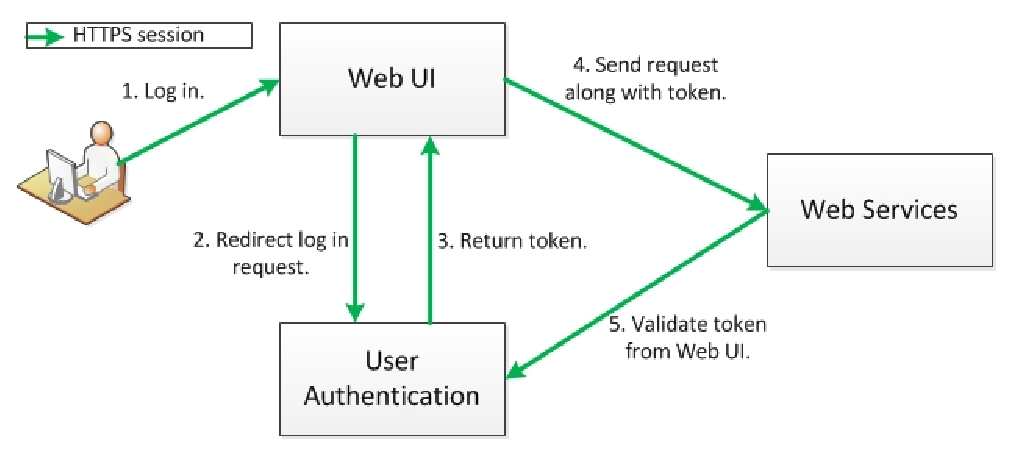
\includegraphics[scale=0.5]{figures/workflow-authentication}
  \caption{Authentication flow.}
  \label{fig:auth}
\end{figure}

\subsubsection{Virtual machine access}

Section \ref{subsubtitle:control} presents an overview of different VM operations. This section focuses on the mechanism we provide to user to access VM. There are two possibilities that copyrighted data may leak from our system during user access. One of them is through network. For one VM, we intend to block arbitrary network access when a user accesses copyrighted data, while keeping network open for the user to download and configure software environment when she does not access copyrighted data. The data capsule provides two VM mode, i.e. maintenance mode and secure mode, to support different network control for the same VM. In maintenance mode, user can access network without any constrains, although the HTRC data service is blocked by firewall policy. In secure mode, user can only access HTRC data service. Any other network accesses are denied. Figure \ref{fig:vmaccess} gives an example. First user creates and starts a VM through the web UI as described in section \ref{subsubtitle:control}. After the VM is up and running, the user can log in to it through any VNC client with proper information provided from web UI, e.g., host name and port number. Note that VNC session is the only channel that user can access VM in secure mode. We block SSH traffic, which is a typical way to access VM in most cloud platforms e.g., Amazon EC2, OpenStack, because it allows user to copy data out by scp command. By default, user logs into VM in maintenance mode. User can install software from internet, upload programs from her desktop, and etc. If user wants to access HTRC Data service, she needs to switch VM mode from maintenance to secure through web UI. In practice, VNC screen will be frozen for a short time (usually 2 to 5 seconds) during the mode switch. In secure mode, user does not have network access except for HTRC Data service.

The other possibility of copyrighted data leakage is to copy data from secure mode to maintenance mode in local disk and leak through network in maintenance mode. In secure mode, copyrighted data may be copied from HTRC Data service in local disk. When VM is switched to maintenance mode, the copyrighted data in local disk is visible in maintenance mode and can be copied out through network. To prevent such leakage, data capsule checkpoints VM image before it goes to secure mode. That is to take a snapshot of the VM by using qemu command. When VM switches from secure mode to maintenance mode, data capsule restores the checkpoint, i.e, the snapshot image, through qemu command. Therefore, all the data written to VM local disk in secure mode will be wiped out when VM switches from secure mode to maintenance mode. Meanwhile, to allow user to persist her data in secure mode, data capsule provides a secure volume, which is only visible in secure mode and shown as an external drive to the VM, to let user write data to. The secure volume stores data persistently and will be detached from VM when VM is in maintenance mode.

A typical workflow for a user to access the VM is depicted in figure \ref{fig:vmaccess}. First, the user creates and starts the VM through web UI. Second, user logs in to VM in maintenance mode through VNC client (step 1). Third, user configures software setting through internet (step 2). Forth, user switches VM mode from maintenance to secure, accesses HTRC Data service and writes data to secure volume (step 3, 4).

Final result release??

\begin{figure}[h]
  \centering
  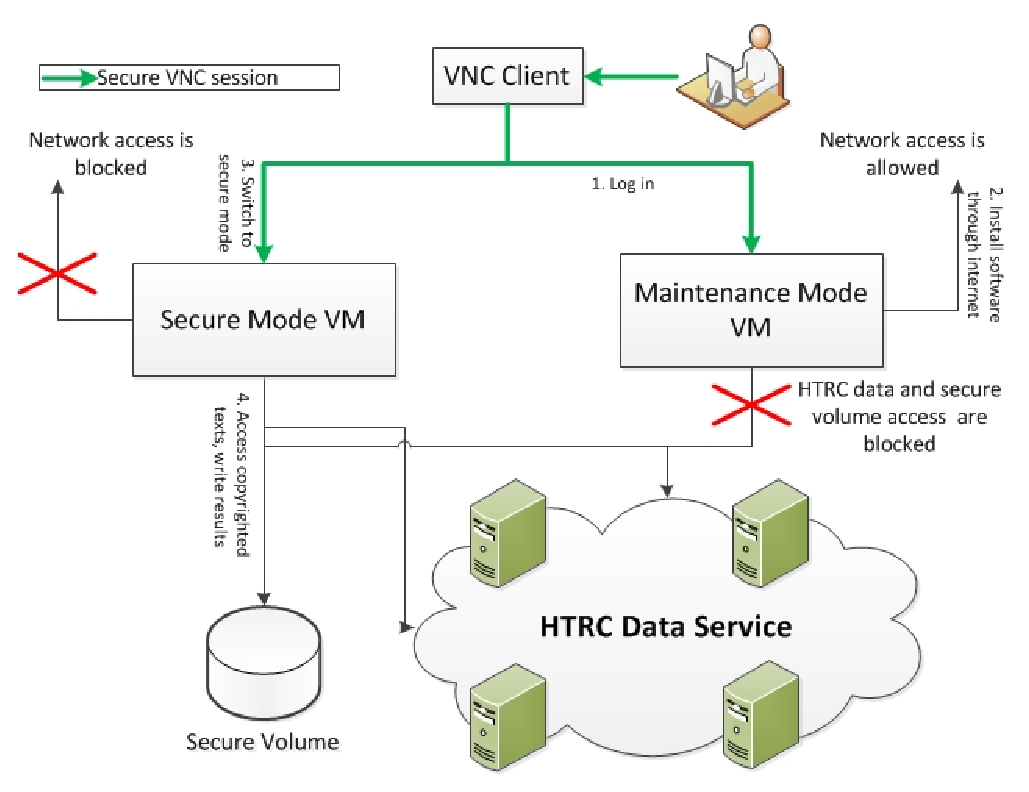
\includegraphics[scale=0.45]{figures/workflow-HTRCData}
  \caption{Virtual machine access flow.}
  \label{fig:vmaccess}
\end{figure}


\subsubsection{Final results review}

Under construction.

In summary, our architecture fulfills the design requirements in section \ref{subtitle:requirement}. First, the web front end and web service use OAuth 2.0 to authenticate user which denies unauthorized users. Second, web service coordinates a number of machines equipped with data capsule to provide a cloud environment and log all user activities. Through the log files, we are able to tell who did what. Third, the data capsule blocks network channels when VM is in secure mode so that no copy out can take place. Forth, researcher can manage and manipulate her virtual machines through a simple web UI which is more user friendly than a command line tool. Besides, researcher can log in to virtual machine through VNC which provisions GUI desktop instead of terminal. In addition, researcher is allowed to configure the hardware setting when creating the VM from web UI and software setting in VM in maintenance mode to meet her needs. These effects help lower the usage burdens for digital humanities researchers. Last but not least, the web service can setup a Hadoop cluster for researcher to run MapReduce jobs although more efforts are needed to configure data capsule properly in a MapReduce context. We leave it as future work.

\subsection{Implementation Details}

\subsubsection{Physical layer implementation}
Under construction.


\subsubsection{Web service layer implementation}
The web service is implemented as an asynchronous Restful service in Jersey framework []. Since operations in hypervisor layer usually take some time to finish, we decouple the response and actual execution to provide good responsiveness. For instance, when a start VM request arrives, web service returns \emph{start-pending} as VM state immediately rather than waits until VM startup finishes and returns \emph{start} state. The web service also takes into account failover on hypervisor layer. It automatically retries connection failure and timeouts long running ssh session. The web service is implemented in a multi-threaded way so that multiple operations on different VM can happen simultaneously.


\section{Future Work} \label{title:future}
We are in the process of implementing final results review mechanism. Once that part is in place, we expect to release our system to humanities researchers for use and get feedbacks from them. There are numerous next steps we can take. First, we intend to build MapReduce cluster automatically with data capsule in place to expand the utilization of data capsule. Second, we are interested in providing researchers with extractive features that comply with non-consumptive research policy. Potential qualified features include word frequency, term document matrix, etc. Third, we will investigate the approach of adding random noises to final result so that user is unable to reconstruct original texts while the accuracy of final results is bounded. For example, after adding noises, the lower bound of accuracy is 90\% which may be sufficient enough to researchers.

\section{Conclusion} \label{title:conclusion}

This paper proposes a cloud framework which complies with non-consumptive research policy to facilitate digital humanities research. The framework is built on top of data capsule and data capsule is extending to adapt to a cloud environment.  We present design details of the framework along with implementation details. Most parts of the system are implemented. We are in the process of implementing the final result review mechanism and plan to release our system to digital humanities researchers in the next couple of months.


%ACKNOWLEDGMENTS are optional
\section{Acknowledgments}

%
% The following two commands are all you need in the
% initial runs of your .tex file to
% produce the bibliography for the citations in your paper.
\bibliographystyle{abbrv}
\bibliography{sigproc}  % sigproc.bib is the name of the Bibliography in this case
% You must have a proper ".bib" file
%  and remember to run:
% latex bibtex latex latex
% to resolve all references
%
% ACM needs 'a single self-contained file'!
%
%APPENDICES are optional
%\balancecolumns

% That's all folks!
\end{document}
